% -*-coding: utf-8 -*-
\documentclass[oneside,11pt,a4paper]{report}

\newif\ifrelease % new boolean variable release. True = include some fancy content
\releasefalse % and set it

\usepackage[czech]{babel}
\usepackage[utf8]{inputenc}
\usepackage[IL2]{fontenc}

\usepackage{amsmath}
\usepackage{amsthm}
\usepackage{amstext}
\usepackage{amsfonts}
\usepackage{epsfig}
\usepackage{graphicx}
\usepackage{color}
\usepackage{multirow}
\usepackage{booktabs}
\usepackage[abs]{overpic}
\setlength\unitlength{1mm}
\usepackage{fancyvrb}
\usepackage{dcolumn}

\usepackage[justification=centering]{caption}
\ifrelease
	\usepackage{pdfpages}
\fi
\usepackage[pagebackref=true]{hyperref} % tento balicek by mel byt na konci baliku!

\hypersetup{
	pdfauthor={Ladislav Horký},
	pdftitle={Celočíselné optimalizační heuristiky a jejich paralelizace}
}

%% Nastavení zrcadla sazby
\usepackage{calc}
\setlength{\textheight}{\paperheight -3cm -3cm}  % horni a dolni okraje 3cm, do tech se musi vejit header a footer
\setlength{\textwidth}{\paperwidth -3.5cm -2.6cm}  % levy okraj 3,5cm (na vazbu), pravy okraj 2,5cm
\setlength{\oddsidemargin}{3.5cm -1in}
\setlength{\topmargin}{(\paperheight-\textheight-\headheight-\headsep-\footskip)/2 - 1in}
%\usepackage{calc}
%\setlength{\textheight}{9in}
%\setlength{\textwidth}{6in}
%\setlength\oddsidemargin{(\paperwidth-\textwidth)/2 - 1in}
%\setlength\evensidemargin{(\paperwidth-\textwidth)/2 - 1in}
%\setlength\topmargin{(\paperheight-\textheight-\headheight-\headsep-\footskip)/2 - 1in}

\parindent=6pt % odsazení 1. řádku odstavce
\parskip=4pt   % mezera mezi odstavci

\ifrelease
	\hypersetup{pdfborder={0 0 0}} % no borders around links
\else
	\hypersetup{colorlinks=true} % colour links instead of borders
\fi
% =========================================================
% Ams definice

\theoremstyle{plain}
\newtheorem{define}{Definice}
\newtheorem{theo}{Věta}


% Vlastní příkazy:==========================================
\newif\ifshownotes % zobraz poznámky level 1
\shownotestrue
\newif\ifshownotesadd % zobraz poznámky level 2
\shownotesaddtrue

\newcommand{\LAs}{\L A_{sqrt}}
\newcommand{\rl}{\textup{(}}
\newcommand{\rr}{\textup{)\,}}
\ifshownotes
    \newcommand{\note}[1]{{\color{green}{\emph{#1}}}}
\else
    \newcommand{\note}[1]{}
\fi
\ifshownotesadd
    \newcommand{\notea}[1]{{\color{green}{\emph{#1}}}}
\else
    \newcommand{\notea}[1]{}
\fi
\newcommand{\LL}{\mathbf{L}}
\newcommand{\sqr}{\mathrm{sqrt}}
\newcommand{\LAsq}{$\mathrm{\L A_{sqrt}}$ }
\newcommand{\beq}{\begin{equation}}
\newcommand{\eeq}{\end{equation}}
\newcommand{\xx}{\mathbf{x}}
\newcommand{\yy}{\mathbf{y}}
\newcommand{\f}{\mathrm{f}}
\newcommand{\g}{\mathrm{g}}
\newcommand{\PP}{\mathcal{P}}
\newcommand{\QQ}{\mathcal{Q}}
\newcommand{\NN}{\mathcal{N}_{R}(x_{i,j,k})}
\newcommand{\MM}{\mathcal{M}_R}
\newcommand{\Lw}{{\mathrm{L^w}_{i,j,k}}}
\newcommand{\Nb}{{\mathrm{N}_{i,j,k}}}
\newcommand{\WL}{{\mathrm{WL}_{i,j,k}}}
\newcommand{\EE}{\mathrm{E}}
\newcommand{\DD}{\mathrm{D}}
\newcommand{\OO}{\mathrm{O}}
\newcommand{\CC}{\mathrm{C}}
\newcommand{\MED}{\mathrm{MED}}
\newcommand{\BES}{\mathrm{BES}}
\newcommand{\kk}{\textit{k}}
\newcommand{\ccc}{\textit{c}}
\newcommand{\et}{\;\,\mathrm{et}\;\,}
\newcommand{\Cpp}{C\raisebox{0.15ex}[0ex][0ex]{++}}

\newcommand{\Nn}{\mathbb{N}}
\newcommand{\RR}{\mathbb{R}}
\newcommand{\Imageman}{{\tt ImageManager<imDataType>}}
\newcommand{\Imageinfo}{{\tt ImageInfo}}
\newcommand{\imDataType}{{\tt imDataType}}
\newcommand{\Analyze}{Analyze$^{\mathrm{\textsc{tm}}}$ 7.5}
\newcommand{\image}{{\tt image}}
\newcommand{\imageGpu}{{\tt imageGpu}}
\newcommand{\bl}[1]{\textcolor[rgb]{0,0,1}{#1}} % prostě fancyverbatim neumí textbf
\newcommand{\cy}[1]{\textcolor[rgb]{1,0,1}{#1}}
\newcommand{\FERMI}{FERMI$^{\mathrm{\textsc{tm}}}$}
\newcommand{\Vr}{\Verb[commandchars = \\\{\}]}
\newcommand{\OOO}{$\mathcal{O}$}

\newcolumntype{d}{D{,}{,}{4.2}}
\newcolumntype{k}{D{,}{,}{2}}
\newcolumntype{j}{D{,}{,}{1}}
\newcolumntype{u}{D{,}{,}{0}}

% Definice makra pro české uvozovky:
\def\bq{\mbox{\kern.1ex\protect\raisebox{-1.3ex}[0pt][0pt]{''}\kern-.1ex}}
\def\eq{\mbox{\kern-.1ex``\kern.1ex}}
\def\ifundefined#1{\expandafter\ifx\csname#1\endcsname\relax }%
\ifundefined{uv}%
        \gdef\uv#1{\bq #1\eq}
\fi

\DeclareGraphicsExtensions{.pdf}

% Dělení slov:=============================================
\hyphenation{pře-klá-da-jí-cí}

% =========================================================
\begin{document}

\ifrelease
	% -*-coding: utf-8 -*-
\newcommand{\cvut}{České Vysoké Učení Technické v~Praze}
\newcommand{\fjfi}{Fakulta Jaderná a Fyzikálně Inženýrská}
\newcommand{\km}{Katedra matematiky}
\newcommand{\obor}{Inženýrská Informatika}
\newcommand{\zamereni}{Softwarové Inženýrství a Matematická Informatika}

\newcommand{\nazevcz}{Paralelní implementace fuzzy filtrů ve zpracování obrazu na GPU}
\newcommand{\nazeven}{Parallel Implementation of Fuzzy Filters in Image Processing on GPU}
\newcommand{\autor}{Ladislav Horký}
\newcommand{\rok}{2011}
\newcommand{\vedouci}{Ing. Tomáš Oberhuber Ph.D.}

\newcommand{\pracovisteVed}{Katedra matematiky \\
    České Vysoké Učení Technické v~Praze}
\newcommand{\konzultant}{doc. Ing. Jaromír Kukal Ph.D.}
\newcommand{\pracovisteKonz}{Katedra softwarového inženýrství \\
    České Vysoké Učení Technické v~Praze}

\newcommand{\klicova}{Fuzzy logika, zpracování obrazu, robustní filtry, GPGPU, CUDA}
\newcommand{\keyword}{Fuzzy Logic, image processing, robust filters, GPGPU, CUDA}
\newcommand{\abstrCZ}{

    Cílem práce bylo zjistit možnosti urychlení filtrace 3D medicínských dat na GPU u obrazových filtrů postavených na fuzzy logice. Nejprve bylo provedeno zobecnění použité teorie do 3D a následná implementace na CPU v jazyce \Cpp ~při použití nejlepších dostupných algoritmů. Implementace na GPU byla provedena v prostředí NVIDIA CUDA C a použité algoritmy a optimalizace jsou až na jeden původní. Hodnoty urychlení jsou na celé škále 2,3krát až 60krát (kde jsme naráželi na pro hardware nevhodné rozměry zpracovávaných dat) a u jednodušších filtrů tak došlo ke zkrácení doby výpočtu na testovacích datech na jednotky ms. Navíc byla provedena teoretická diskuse schopnosti filtrů medián, BES, H.-L. medián a WBES odstraňovat kontaminovaný gaussovský šum i s praktickými příklady.}
\newcommand{\abstrEN}{

    The aim of the thesis was to determine the possibility of speeding up 3D medical image processing on GPU using filters based on Fuzzy logic. First, generalization of the theory into 3D and subsequent implementation on CPU using \Cpp ~language and the best possible algorithms was carried out. Implementation on GPU was made within the NVIDIA CUDA C enviroment with all but one used algoritms and optimizations being original. The gained speedup ranges from nearly 60 times down to 2,3 times (where most difficulties with input data dimensions occured) and the total duration of computation dropped for some filters below 10 ms. As a bonus, a theoretical discussion on median, BES, H.-L. median and WBES capability of suppressing contaminated gaussian noise together with practical expamples were carried out.}

%%% zde zacina kresleni dokumentu

% titulní strana
\thispagestyle{empty}

\begin{center}
	{\Large  \bf  \cvut\\[2mm] \fjfi }
	\vspace{10mm}

	\begin{tabular}{c}
	{\bf \km}\\
	{\bf Obor: \obor}\\
	{\bf Zaměření: \zamereni}
	\end{tabular}

	\vspace{10mm} \epsfysize=20mm  \epsffile{cvut-logo-bw-600} \vspace{15mm}

	{\LARGE
	\textbf{\nazevcz}
	\par}

	\vspace{5mm}

	{\LARGE
	\textbf{\nazeven}
	\par}

	\vspace{30mm}
	{\Large BAKALÁŘSKÁ PRÁCE}

\end{center}

\vfill
{\large
\begin{tabular}{rl}
Vypracoval: & \autor\\
Vedoucí práce: & \vedouci\\
Rok: & \rok
\end{tabular}
}

% zadání bakalářské práve
\newpage
\thispagestyle{empty} Před svázáním místo téhle strany \fbox{vložíte zedání práce} s podpisem
děkana (bude to jediný oboustranný list ve Vaší práci) !!!!

% prohlášení
\newpage
\thispagestyle{empty}
~
\vfill


{\bf Prohlášení}

\vspace{0.5cm}
Prohlašuji, že jsem svou bakalářskou práci vypracoval samostatně a použil jsem pouze podklady
(literaturu, projekty, SW atd.) uvedené v přiloženém seznamu.

\vspace{5mm}V Praze dne ....................\hfill
    \begin{tabular}{c}
    ........................................\\
    \autor
    \end{tabular}

% poděkování
\newpage
\thispagestyle{empty}
~
\vfill

{\bf Poděkování}

\vspace{5mm}
Rád bych poděkoval panu Ing. Tomáši Oberhuberovi Ph.D. a panu doc. Ing. Jaromíru Kukalovi Ph.D. za podporu, velkou vstřícnost a cené rady a zkušenosti, které mi při vedení práce a konzultacích v bohaté míře poskytovali.

\begin{flushright}
\autor
\end{flushright}

% strana s abstraktem
\newpage
\thispagestyle{empty}

\newbox\odstavecbox
\newlength\vyskaodstavce
\newcommand\odstavec[2]{%
    \setbox\odstavecbox=\hbox{%
         \parbox[t]{#1}{#2\vrule width 0pt depth 4pt}}%
    \global\vyskaodstavce=\dp\odstavecbox
    \box\odstavecbox}
\newcommand{\delka}{120mm}

\hspace{-0.9cm}
\begin{tabular}{ll}
  {\em Název práce:} & ~ \\
  \multicolumn{2}{l}{\odstavec{\textwidth}{\bf \nazevcz}} \\[5mm]
  {\em Autor:} & \autor \\[5mm]
  {\em Obor:} & \obor \\
  {\em Druh práce:} & Bakalářská práce \\[5mm]
  {\em Vedoucí práce:} & \odstavec{\delka}{\vedouci \\ \pracovisteVed} \\[5mm]
  {\em Konzultant:} & \odstavec{\delka}{\konzultant \\ \pracovisteKonz} \\[5mm]
  \multicolumn{2}{l}{\odstavec{\textwidth}{{\em Abstrakt:} ~ \abstrCZ \\ }} \\[5mm]
  {\em Klíčová slova:} & \odstavec{\delka}{\klicova} \\[20mm]

  {\em Title:} & ~\\
  \multicolumn{2}{l}{\odstavec{\textwidth}{\bf \nazeven}}\\[5mm]
  {\em Author:} & \autor \\[5mm]
  \multicolumn{2}{l}{\odstavec{\textwidth}{{\em Abstract:} ~ \abstrEN \\ }} \\[5mm]
  {\em Key words:} & \odstavec{\delka}{\keyword}
\end{tabular}
 % úvodní strany
\fi
    \newpage
    \pagenumbering{roman}
    \tableofcontents

    \chapter*{Úvod}
    \pagenumbering{arabic}
        \addcontentsline{toc}{chapter}{Úvod}
        % -*-coding: utf-8 -*-

% cíl, trend

% aplikace zpracovává 3D obraz

Práce je zaměřená na urychlení známých obrazových filtrů na GPU. Přesouvání výpočtů na GPU má dnes už ve vědecké komunitě své pevné místo a k řadě problémů, jako např. třídění polí a konvoluce v obraze, jsou již k dispozici knihovny GPU využívající. Náš problém se však menšími rozměry vstupních dat -- je třeba třídit pole pouze o stovkách prvků -- tomuto mainstreamu poněkud vymyká. Algoritmy, které urychlí fitraci na dobu milisekund až desítky milisekund mohou být výhledově použity v aplikacích, které potřebují výsledky filtrů v reálném čase. To může být naříklad program s okamžitou vizuální zpětnou vazbou, umožňující laikovi sestavit si potřebný filtr pomocí jednoduchého skládání filtrů a manipulací s jejich parametry.

Jako teoretický základ filtrů byla použita fuzzy logika, konkrétně \L ukasiewiczova algebra s odmocninou, která je přímo aplikovatelná na data tak, jak jsou v počítači reprezentována a je vhodná pro konstrukci sítí filtrů, při jíž se může urychlení na GPU taktéž bohatě uplatnit.
Popis je zaměřen na typové filtry ze tříd morfologický a statisticky motivovaných filtrů, které jsou posléze i implementovány.

V práci nebudeme porovnávat urychlení konkrétních algoritmů mezi CPU a GPU, ale urychlení celých filtrů. Při implementaci jsou tak na CPU a GPU použity pro ten samý filtr vždy rozdílné algoritmy, z nichž každý je optimalizován na rychlost a konkrétní platformu -- díky hardwarovým omezením na GPU klademe na kód jiné požadavky.

Implementace na CPU je provedena v jazyce \Cpp ~za použítí nejlepších dostupných algoritmů, na GPU je použito prostředí NVIDIA CUDA C a použité algoritmy a optimaliazce jsou až na výjimky původní.

Za svůj autorský podíl na práci považuji sjednocení symboliky v rešeršní části práce a diskusi citlivosti filtrů na kontaminovaný gaussovský šum. Dále pak návrh a realizaci programu pro testování urychlení filtrů na GPU v prostředí CUDA C a diskusi problematiky třídění malých polí na GPU.


    \chapter{Přehled optimalizačních algoritmů}
        % -*-coding: utf-8 -*-

V této kapitole popíšeme několik vybraných optimalizačních algoritmů. Zdaleka nejde o průřez všemi typy algoritmů\footnote{obsáhlejší přehledy lze nalézt například v \cite[p.~23]{GO ebook}, \cite{wiki metaheur}}, ale alespoň získáme představu s čím se budeme muset při hledání obecného formalismu potýkat. Na konci zmíníme obecné principy, myšlenky a problémy, které se objevují napříč všemi algoritmy, a které bychom taktéž chtěli pokrýt.

\section{Základní pojmy}

\par{\textbf{Účelová funkce (fitness)} je funkce, jejíž hodnotu se algoritmus snaží optimalizovat. Optimalizaci lze vždy formulovat jako minimalizaci.}

\par{\textbf{Kandidátní řešení (jedinec)} je struktura dat, z nichž je možné spočíst hodnotu účelové funkce. Manipulací s těmito daty se algoritmus snaží najít nejlepší možné řešení.}

\par{\textbf{Stavový prostor} je prostor všech jedinců.}

\par{\textbf{Populace} je soubor jedinců s nimiž algoritmus aktuálně pracuje. Ne každý algoritmus potřebuje populaci}

\par{\textbf{Krok algoritmu}} posloupnost operací, která má za následek přechod k novému jedinci, případně nové generaci. Posloupnost operací je v každém kroku stejná.

\par{\textbf{Metaheuristika} je obecný návrh algoritmu popisující myšlenky, jakými budeme jedince krok po kroku zlepšovat aniž bychom dělali složitější předpoklady o účelové funkci, charakteru problému nebo implementaci. Myšlenky obsažené v metaheuristice zřídkakdy zajišťují konvergenci algoritmu k optimálnímu řešení.}

\section{Algoritmy}

Pokud není řečeno jinak, u algoritmů vždy popisujeme jeden jejich krok a vynecháváme ukončující podmínku, kterou bývá často konvergence algoritmu, nebo dosažení dostatečně nízké fitness.

\subsection{Simulované žíhání a zrychlené simulované žíhání}

\textbf{Simulované žíhání} (SA -- Simulated Annealing) \cite{SA Hajek}, \cite{SA Tsitsiklis} je metaheuristika založená na analogii s chladnutím kovu. Při chladnutí se atomy snaží zaujmout pozici s co nejnižší potenciální energií; když je teplota vysoká, Brownův pohyb je intenzivní a atomy se často dostávají i do stavů s vyšší energií než měly dříve, což jim umožňuje uniknout z lokálních minim potenciální energie. Naproti tomu při nízké teplotě se atomy pohybují již téměř výhradně do stavů s nižší energií. Správnou rychlostí ochlazování (cooling schedule) Pak můžeme dosáhnout ideálně homogenního krystalu kovu, nebo alespoň velkých zrn.

V konkrétním popisu algoritmu se různé prameny liší (srov. \cite{SA Hajek}, \cite{VFSA}). Rozdíly popíšeme, ale pro vysvětlení se přidržíme první z definic \note{\cite[p.~1153]{SA survey}}. Nechť jsme ve stavu $x_i$:
\begin{enumerate}
  \item $x_{new} \in N(x_i)$, kde $N(x)$ je pevné okolí stavu $x$.
  \item Pokud $E(x_{new}) < E(x_i) \quad\Rightarrow\quad x_{i+1} \leftarrow x_{new}$,
  \item jinak $x_{i+1} \leftarrow x_{new}$ s pravděpodobností $p(\Delta E,T_i) = exp(-\frac{E(x_{new}) - E(x_i)}{T_i})$,
    \newline kde $T_i = \frac{T_0}{ln(i)}$, $i$ je krok.
  \item Je-li splněna podmínka pro konec (např. dosažení cílové teploty) skonči, jinak \linebreak $i\leftarrow i+1$ pokračuj na 1.
\end{enumerate}

%\note{různé prameny uvádějí různé přístupy: např. u \cite{VFSA} je mutace i pravd. příjmu parametrizovaná teplotou -- takže je to vlastně quantum SA a důkazy konvergence nejsou vedeny přes přijímací pravd, ale přes mutaci. Na druhou stranu, důkazy v Hájkovi a Tsitsiklisovi jsou vedeny přes přijímací pravd. a předpoklady o okolí jsou poměrně volné...}

V \cite{SA Hajek}, \cite{SA Tsitsiklis} je dokázáno, že pro dostatečně vysoké $T_0$, při daném postupu ochlazování $x_i \xrightarrow{i \to +\infty} x_{opt}$ podle pravděpodobnosti. Zastavení algoritmu určujeme volbou cílové teploty (běžně i řádu $10^{-4}$) z čehož vyplývá okamžitá nevýhoda SA a tou je v praxi příliš pomalý pokles teploty.

Zmíněné rozdíly se týkají toho, že některé články \cite{SA survey},\cite{VFSA} zavádějí závislost teplotě i do funkce okolí, $N(x,T_i)$ má pak nejčastěji tvar pravděpodobnostního rozdělení s $x$ jako střední hodnotou a teplota ovlivňuje rozptyl, nebo plochost rozdělení. Důkaz konvergence se pak vede přes funkci okolí a je o něco jednodušší. Tento přístup se pro podobnost s tunelovým jevem často nazývá Kvantové simulované žíhání (QSA).

\textbf{Rychlé simulované žíhání} (FSA) \cite{VFSA} je odpovědí na praktický problém, že pokles teploty u SA je příliš pomalý. Z důkazů konvergence plyne, že můžeme volit rychlejší cooling schedule, pokud zvolíme jinou přijímací pravděpodobnost $p(\Delta E,T_i)$ (nebo funkci okolí u QSA). FSA pracuje s rychlejším -- inverzně lineárním -- cooling schedule, při pevném okolí má pak $p(\Delta E,T_i)$ tvar kvantilu z Cauchyho rozdělení, v případě QFSA funkce okolí nemá normální, ale Cauchyovské rozdělení umožňující občasné velké skoky.

\note{článek od Szu nemůžu sehnat.... na Esevieru jako jediný nemá pdf...}

\subsection{Genetická optimalizace}

Genetická optimalizace je podtřída obecnějších \emph{evolučních algoritmů} a je inspirovaná křížením genů v přírodě. Přesnou terminologií se zabývat nebudeme, její popis lze nalézt např. v \cite[p.~141]{GO ebook}. Jedná se o populační algoritmus jehož jedinci jsou reprezentováni binárními řetězci, což můžeme v našem případě zobecnit na celočíselné řetězce. Na rozdíl od SA a FSA vzniká nový jedinec z více, typicky dvou jedinců z minulé generace. Po počáteční náhodné inicializaci se průběh GO dá popsat následujícím schématem:

\begin{figure}[h!]
  \includegraphics[width=\textwidth]{img/EA}
  \caption{Schéma genetické optimalizace}\label{EA fig}
\end{figure}

\subsubsection{Selekce}

Selekce je odrazem selekce přírodní a stará se o to, aby byli kříženi hlavně dobří jedinci. Častou podmínkou na tento výběr je, aby jedinci vybraní ke křížení nebyli totožní. Konkrétních způsobů je mnoho, všechny jsou přirozeně stochastické. Jako příklad uvedeme základní ruletové kolo (roulette wheel) a turnajovou selekci (tournament selection).

V případě ruletového kola je pravděpodobnost výběru $i$-tého jedince rovna $p_i = f_i/\sum_{j \in P} f_j$, tedy relativní fitness jedince. Tento způsob je jednoduchý, avšak velmi citlivý na rozdělení fitness v populaci: pokud bude mít jeden jedinec řádově lepší fitness než ostatní, můžeme se v další generaci dočkat zhuštění potomků právě kolem tohoto jedince a následné předčasné konvergence algoritmu.

Turnajová selekce se snaží tuto vadu odstranit: nejprve je náhodně vybráno $k$ ($k\geq 2$) jedinců a z nich je vybrán ten s nejlepší fitness. Při nízkých $k$ tak dostanou šanci i horší kandidáti. Více o způsobech selekce v \cite{GO ebook}.

\subsubsection{Křížení}

Křížení vytváří nového jedince (řetězec) v případě GO kombinací dvou jedinců z předchozí generace tak, že:
\[
\begin{split}
z_i = x_i &\quad\text{pro}\quad i \in I \\
z_i = y_i &\quad\text{pro}\quad i \in \text{\^{n}}\backslash I
\end{split}
\]
kde $n$ je délka řetězce a množina $I$ závisí na typu křížení -- to může být jednobodové ($z$ obsahuje jeden souvislý podřetězec z $x$ a jeden z $y$), vícebodové, nebo s maskou. V případě celočíselných řetězců může být křížením např. i zaokrouhlená lineární kombinace $x$ a $y$. 

V některých algoritmech vzniká nový jedinec křížením jen s jistou pravděpodobností. Zbytek potomstva je pak doplněn prostou selekcí z populace.

\subsubsection{Mutace}

Křížením získaný jedinec je s jistou pravděpodobností zmutován (opět srovnání s přírodou). V případě, že křížení je pouhou kombinací podřetězců, je mutace jediný způsob, jak do řetězců (potažmo do populace) vnést nové hodnoty. Způsobů mutace je opět mnoho: k řetězci může být přičten Gaussovský, nebo Cauchyovský šum a výsledek zaokrouhlen na celá čísla. U binárních řetězců se často používá změna náhodného prvku řetězce.

\subsubsection{Nová generace}

Při GO je nejčastěji $N = |P| \geq |Q|$. Nová populace $P_{i+1}$ se pak vytvoří z $N$ nejlepších potomků z $Q$, nebo z $N$ nejlepších z $P \cup Q$. Způsobů je opět více, může být uplatněn například elitismus (viz \ref{myslenky GO}).

\subsection{Diferenciální evoluce}

Diferenciální evoluce \cite{DE Storn} je optimalizační algoritmus vhodný pro mnohodimenzionální stavové prostory a byl navržen jako diskrétní alternativa algoritmů vyžadujících spojitost a existenci derivace účelové funkce. Je opět ze třídy evolučních algoritmů, jen reprodukce je o něco složitější než u GO (viz obrázek \ref{DE fig}).

\begin{figure}[h!]
  \includegraphics[width=\textwidth]{img/DE}
  \caption{Schéma diferenciální evoluce}\label{DE fig}
\end{figure}

Nejprve je z náhodných jedinců $a \ne b \ne c \; (\ne x)$ vytvořena lineární kombinace s \linebreak $F \in [0,2]$ jako zesilovacím činitelem diference. Rozdíl vektorů nahrazuje derivaci a snaží se reprezentovat \bq trend poklesu\eq   fitness. Takto vytvořený vektor $y$ je pak klasicky zkřížen s vektorem $x$ a výsledek může být ještě zmutován. Fitness výsledného vektoru $x_{new}$ je pak srovnána s fitness $x$ a pokud je nižší, je $x$ v populaci nahrazen $x_{new}$. Toto postupně provedeno pro všechny vektory v populaci. Je zřejmě, že nutně $|P| > 4$, abychom mohli vybrat různé vektory.

\subsection{Evoluční strategie}

Evoluční strategie \cite{ES comprehensive},\cite{GO ebook} jsou podtřídou evolučních algoritmů a jedná se o jedny z prvních evolučních algoritmů. Na rozdíl od předchozích se ale spoléhají pouze na mutaci a selekci a neobsahují křížení -- mutace je často Gaussovská, selekce je dána velikostí populace a potomstva ($|P|$ a $|Q|$) a způsobem, jakým se tvoří nová populace $|P_{i+1}|$.

Podle toho existuje několik variant, například (1+1)-ES, ($\mu$+1)-ES, ($\mu$+$\lambda$)-ES a ($\mu$,$\lambda$)-ES, kde $\lambda \geq \mu$. První číslo určuje velikost populace ($|P|$), druhé velikost potomstva ($|Q|$). Znaménko \bq +\eq   značí, že nová populace vznikne výběrem nejlepších jedinců z $P\cup Q$, \bq ,\eq   naopak, že stará populace bude nahrazena výběrem nejlepších pouze z $Q$. Podrobnější informace o ES lze najít v \cite{ES comprehensive}.

ještě to o pravidle 1/5?... změně mutace, CMAES?

\section{Dílčí principy optimalizačních algoritmů}\label{myslenky GO}

\subsection{Globální VS lokální hledání}

Neboli diverzifikace versus intenzifikace. Jsou dvě hranice mezi nimiž se optimalizační algoritmy pohybují. Globální prohledávání se snaží co nejrovnoměrněji navzorkovat celý stavový prostor (dostat jedince v populaci co nejdále od sebe) a jeho průběh prakticky nezávisí na předchozích stavech algoritmu. Ten se tak efektivně vyhne uvíznutí v lokálním minimu, avšak nemá šanci vylepšit případné slibné jedince. Globálním prohledáváním nelze tedy dosáhnout optimální výsledku, jeho výkonnost je však zcela nezávislá na charakteru účelové funkce. Typickým příkladem čistě globální heuristiky je náhodné prohledávání.

Lokální prohledávání naopak jedince po malých krocích stále vylepšuje. Pokud již jedinec vylepšit nejde (v okolí není žádný s nižší účelovou funkcí), skončí. Chová se tedy přesně opačně než globální prohledávání -- zákonitě uvízne v každém globálním minimu, ale jedince \bq vytěží\eq na maximum. Pro jiné, než unimodální účelové funkce také nedává optimální řešení. Jeho příkladem je například Shoot\&Go (Hill-climbing).

Protože žádný z přístupů není optimální, snaží se je algoritmy vhodně staticky, nebo adaptivně kombinovat.

\subsection{Elitismus}

Tento pojem se zrodil u evolučních algoritmů a je pokusem, jak v populaci implementovat lokální prohledávání. U EA se často při přechodu do nové generace celá populace zahodí a nahradí se potomstvem, nebo jeho částí. Tím se však vzdává šance podrobněji prozkoumat okolí dobrých jedinců. Proto se při tvorbě nové populace nechávají nejlepší jedinci (elita, jednotky procent z populace) do další generace, čímž se částečně lokalita zabezpečí. Při neopatrnosti (mnohočlenná elitá) to však může vést k předčasné konvergenci algoritmu.

V návaznosti na elitismus by se dal zavést i komplementární pojem \emph{ostrakizace}\footnote{vyloučení ze středu}, kdy se před dalším krokem vezme nejhorší část populace a nahradí se náhodně inicializovanými jedinci. To například provádí (i když bez tohoto označení) algoritmus Cuckoo Search (kukaččí hledání) \cite{cuckoo}.

\subsection{Parazitismus}

Parazitizmus je komplement elitismu pro algoritmy využívající křížení. Při použití ostrakizace zahazujeme celého jedince a tedy jeden výpočet účelové funkce přijde na zmar. Náhodně vygenerovaný jedinec navíc bývá velmi suboptimální. Pokud trvá výpočet účelové funkce řádově déle než zbytek algoritmu, tento postup si nemůžeme dovolit a při implementaci diverzifikace se postupuje opatrněji: s určitou pravděpodobností do křížení nevstupují dva kandidáti z populace, ale jeden je nahrazen parazitem -- náhodně generovaným jedincem. Část kvality jedince se tak zachová.

\subsection{Niching}

Niching je další způsob, jak zabránit těsnání jedinců kolem lokálních minim. Spočívá v tom, že po ohodnocení se fitness jedinců opraví o faktor závisející na lokální hustotě jedinců ve stavovém prostoru. Jedinci, kteří jsou blízko sebe budou mít tak vyšší (horší) fitness, než jedinci osamocení, a tedy spíše v další generaci zaniknou. Název pochází od biologického výrazu \emph{nika}, což je vymezení prostoru, který daná populace (druh) zabírá v ekosystému. Tento postup se občas označuje jako použití tzv. \emph{Sharing function}.

\subsection{Žíhání (Annealing)}

Žíhání přímo pomáhá jedincům uniknout z lokálních minim. Je použitelné u algoritmů, kde je vztah rodič-potomek vzájemně jednoznačný a pravděpodobně by šlo zobecnit i na případ, kdy má jeden rodič více potomků, ale potomek má právě jednoho rodiče. Myšlenka pochází z iteračních nepopulačních algoritmů a říká, že jedinec není nahrazen potomkem, jen pokud je onen potomek lepší, ale s jistou pravděpodobností i potomkem horším. Tato pravděpodobnost většinou závisí na tom, o kolik je potomek horší a na řídícím parametru, který s postupem času tuto pravděpodobnost zmenšuje. To zajistí, abychom na konci algoritmu neuvázli právě v onom horším řešení.



    \chapter{Programování na GPU}
        % -*-coding: utf-8 -*-

% Vývoj GPU
% Programovací prostředí
    % CUDA
% Architektura GPU (NVIDIA)
    % Hierarchie paměti
    % Hierarchie paralelizace


%čím rychlejší chceme výpočty, tím více omezneí musíme splnit

%Zatím to vypadá, že klasické qsorty atd. budou mít velké overheady
%Zkusit qsort po warpech a porovnat s tím O(n2), co mám teď, ten taky zjemnit na warpy
%Obecně naplnit sdílenou paměť, něco jako pár threadů na pixel

%    -- je to porovnání s 350 na jeden krok VS porovnání s 32 v jednom z několika kroků + scan sumy

%BES na CPU (rozkrájený quickselect)

V této kapitole se stručně seznámíme s historií a vývojem v oboru výpočtů na GPU, rozebereme vlastnosti, přednosti a nevýhody GPU architektury v porovnání s klasickým CPU a nakonec popíšeme programovací model CUDA\footnote{Compute Unified Device Architecture} od společnosti NVIDIA, který použijeme pro implementaci filtrů na GPU.

\section{Vývoj GPU}

    S použitím GPU pro jiné, než grafické výpočty se začalo experimentovat, jakmile přestaly být grafické karty -- hlavně díky rozvoji herního průmyslu -- pouhým jednoúčelovým zařízením a staly se z nich, alespoň částečně, programovatelné paralelní procesory. Vzhledem k tomu, že karty byly primárně ke zpracování grafiky, daly se výpočty provádět pouze pomocí grafického API například přes textury a programovatelné pixel-shadery, což značně snižovalo efektivitu zpracování díky vysoké režii API.

    Zřejmě první velká společnost, která se rozhodla vyjít vstříc požadavkům na konstrukci GPU jako univerzálně použitelné vysoce paralelní výpočetní jednotky, byla NVIDIA, když změnila celý koncept nově vyvíjeného čipu a zavedla tzv. CUDA-jádra -- obecnější a pružnější, než jednotky dedikované ke specifickým grafickým operacím\footnote{ty jsou ovšem na kartách stále přítomny a lze je v programu pro tyto specifické operace použít (např. výpočet $\sin$, $\cos$)}. V únoru 2007 pak představila první verzi vývojového nástroje CUDA, který umožňoval efektivně využívat hardware GPU pomocí několika rozšíření jazyka C a posléze \Cpp. CUDA-jádra novějších karet dokonce umí počítat nativně v dvojnásobné přesnosti; u běžných karet jsou ale tři čtvrtiny jader pro dvojitou přesnost deaktivovány \cite{Heller} (pro grafické operace nejsou třeba), a pro plný výkon ve dvojité přesnosti si musíme koupit (řádově dražší) kartu ze série TESLA, která je primárně určena pro intenzivní výpočty. Veškerý vývojový software poskytuje NVIDIA zdarma.

    V současnosti existují k CUDA dvě alternativy: prostředí OpenCL\footnote{Open Compute Language}, zaštítěné sdružením Khronos Group, které se profiluje jako standard pro heterogenní paralelní programování a DirectCompute od Microsoftu stojící na balíku DirectX verze 10 a vyšší. Výhodou OpenCL je, že stejný kód lze zkompilovat jak pro CPU, tak pro GPU výrobců ATI a NVIDIA\footnote{jinak se bohužel jedná o vzájemně nekompatibilní technologie}. Z principu tedy nemůže poskytovat tak pohodlný přístup, jako CUDA a výsledkem je poměrně rozsáhlý kód. \emph{Dále se budeme zabývat pouze prostředím CUDA a hardwarem s ním souvisejícím.}

    \subsection{Současnost}

     V současnosti je GPGPU\footnote{General Purpose computation on Graphics Processing Units} již etablovaný obor. Hlavní trend vývoje GPU je nyní podobný, jako v počátcích CPU -- spočívá v odstraňování omezení, která musíme na kód klást, abychom dosáhli optimálního výkonu, a ve větší univerzalizaci hardwaru. Tím pádem se i rozšiřuje množina úkolů vhodných pro zpracování na GPU. Jednotlivé výpočetní jednotky na kartách už dávno nejsou pouhými jednoduchými vektorovými procesory, ale stále více se blíží plnohodnotnému (vícejádrovému) procesoru, i když si samozřejmě svůj vektorový charakter zachovávají. Asi nejvíce je to vidět na práci s pamětí, kde u nejnovějšího čipu \FERMI ~z dílny NVIDIA přibyla vrstva chache, čímž došlo k rozvolnění přístupu do globální paměti (viz dále), ale došlo i k rozdělení vektorového procesoru na dva téměř samostatně fungující díly.

\section{Architektura GPU}

    \subsection{Rozdíly CPU a GPU}

        Nyní se podrobněji podíváme na specifika architektury čipů grafických karet. Hlavní otázkou je, pro jaké úlohy jsou vůbec GPU vhodné. Obrázek~\ref{cpu vs gpu} zhruba ukazuje, jak velká část čipu (DRAM ovšem není přímo na čipu) CPU a GPU je dedikována pro určitý druh operací.

        \begin{figure}[h]
          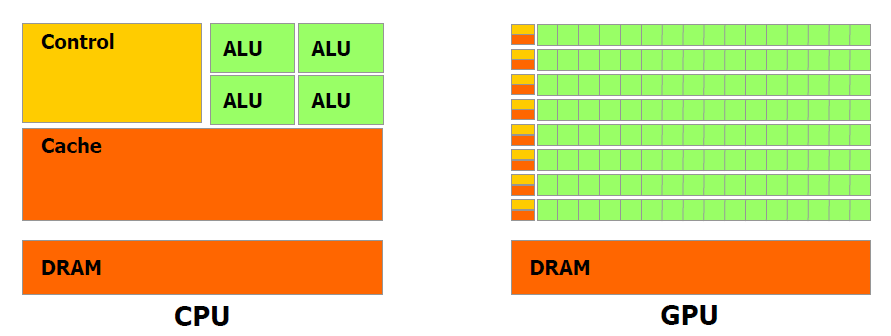
\includegraphics[width = \textwidth]{src/2Gpu/CPUGPU.png}
          \caption{Rozdíly využití čipu na CPU a GPU, převzato z \cite{CUDA programming g.}}
        \end{figure}\label{cpu vs gpu}

        Vidíme, že velkou část čipu CPU zabírá cache a kontrolní logika. Ty zajišťují několika ALU\footnote{Arithmetic Logic Unit} dostatečný přísun dat a instrukcí (např. pomocí hyper-threadingu a branch-prediction), lhostejno jak moc se program větví, nebo jak jsou data uspořádána v DRAM.

        GPU se naproti tomu skládá z několika samostatně funkčních vektorových procesorů -- tzv. SM\footnote{Streaming Multiprocesor} jednotek, z nichž každá má vlastní malou cache a z kontrolní logiky má naprosté minimum. Z toho plyne jednak jistá nutná disciplína při přístupu do DRAM, která je ale narozdíl od té na CPU lépe optimalizovaná na sekvenční čtení, a za druhé musíme běh programu přizpůsobit tomu, že GPU je po částech SIMD\footnote{Single Instruction Multiple Data}, respektive SIMT\footnote{Single Instruction Multiple Thread -- název pocházející od NVIDIA} -- narozdíl od vícejádrového CPU, které je plnohodnotné MIMD\footnote{Multiple Instruction Multiple Data}. Podrobný popis nejnovějšího SM z čipu \FERMI ~lze nalézt v \cite{Fermi}.

        Obecně můžeme říci (protože velká část čipu GPU je dedikována pro aritmetiku), že GPU je nejvíce vhodná pro aritmeticky intenzivní výpočty, tzn. mající vysoký poměr počtu aritmetických operací ku počtu přístupů do paměti.

    \subsection{Algoritmy vhodné pro GPU}

        Před paralelizací algoritmu pro GPU musíme tedy zvážit, zda to má vůbec smysl -- pro dosažení optimálního urychlení musí algoritmus v co největší míře splňovat následující body:
        \begin{itemize}
          \item rozložitelnost výpočtů na nezávislé části, které lze vykonávat paralelně (výsledek jedné nezávisí na výsledku ostatních)
          \item malý počet přístupů do paměti, nejlépe sekvenční/blokové
          \item podobný kód ve všech paralelních částech, minimální a předvídatelné větvení programu
        \end{itemize}

        Jak uvidíme, filtrování obrazu nesplňuje tyto body úplně (např. přístupy do paměti) -- kdyby splňovalo vše, tak se jím nemá příliš cenu zabývat -- ale dostatečně na to, abychom dosáhli použitelných výsledků.

\section{Pogramovací model CUDA a jeho HW implementace}

    \subsection{Úvod}
    Pro maximální efektivitu paralelizace vyvinula NVIDIA několikavrstvou dobře škálovatelnou strukturu s přímou návazností na svůj hardware. Nejmenší výpočetní jednotkou z pohledu programu je \emph{thread} (vlákno), který fyzicky běží na jednom CUDA-jádře v SM. Thready se sdružují do \emph{thread-bloků}, které běží na celém SM a mohou mít 1D, 2D, nebo 3D strukturu, podle toho jakého charakteru jsou zpracovávaná data. Poslední článek tvoří \emph{grid} běžící na celé GPU obsahující (zatím) nejvýše 2D strukturu thread-bloků. Z programu pak výpočty spouštíme pomocí volání \emph{kernelu} obsahujícího náš kód, kterému sdělíme v kolika thread-blocích má běžet, jakou mají mít strukturu v gridu, kolik threadů má být uvnitř thread-blocku a jak mají být uspořádány. To umožňuje ten samý kernel spouštět na různých zařízeních, protože sám hardware rozhoduje, jak jednotlivé výpočetní elementy mezi SM (a posléze CUDA-jádra) rozdistribuuje.

    \subsubsection{Úrovně přístupu}

    Na straně uživatele poskytuje NVIDIA dvě rozhraní: nízkoúrovňové CUDA Driver API a vysokoúrovňové CUDA runtime API, v současnosti ve verzi 4.0. Driver API poskytne uživateli totální kontrolu nad kartou výměnou za složitější a delší kód -- uživatel musí zajistit inicializaci zařízení, přesun dat a funkčních parametrů pro kernel na kartu a přesun a spuštění kernelu samotného. Rozhraní Driver API je v C a funkčně zhruba odpovídá OpenCL. Runtime API je rozšířením C, které umožňuje kernel napsat podobně jako funkci v C a při volání jí speciální syntaxí sdělit, kolik threadů a bloků chceme spustit. O inicializaci a vše ostatní se postará runtime. Nevýhodou Runtime API je, že jeden CPU proces nemůže používat více zařízení, což se ale nové verze snaží vylepšit.

    Mixování obou přístupů (např. právě kvůli použití více zařízení) se nedoporučuje, ale v rozumné míře možné je -- pravidla mixování stanovila až CUDA 4.0. V našem kódu používáme výhradně Runtime API, proto se dále budeme zabývat pouze jí.

    \subsubsection{Výpočetní schopnost}

    Tento termín bude dále v textu často používán. Výpočetní schopnost\footnote{Compute Capability} (VS) udává fyzickou verzi čipu -- všechna CUDA-enabled zařízení před architekturou \FERMI ~mají VS 1.x, čipy s touto architekturou 2.x. Různé VS se liší množsvím paměti, registrů, strukturou SM atd. Největší skok je samozřejmě mezi 1.x a 2.x. Podrobný popis rozdílů mezi VS je k dispozici v \cite[přílohy]{CUDA programming g.}. Pokud budeme dále uvádět konkrétní hodnoty, budou pro VS 1.0, pro kterou je kód primárně optimalizován. Pokud to bude důležité, bude v závorce uvedena hodnota pro VS 2.0. \note{-- na kartách s těmito VS budou totiž i počítány experimentální výsledky.}

    \subsection{Kernel}

    Runtime API nám dovoluje míchat kód pro CPU i GPU v jednom souboru, definici kernelu proto rozlišíme specifikátorem
    \Vr"\cy{__global__}" (příklad převzat z \cite{CUDA programming g.}).

    \begin{Verbatim}[commandchars = \\\{\}]
    // definice kernelu
\cy{__global__} \bl{void} MyVecAdd(\bl{float} *A, \bl{float} *B, \bl{float} *C)\{
    \bl{int} i = \cy{threadIdx}.x;
    C[i] = A[i] + B[i];
\}
    // volání kernelu v programu
    MyVecAdd<<<1,N>>>(A,B,C);
    \end{Verbatim}

    Při volání v příkladu specikujeme, že chceme jeden thread-blok a N threadů jako vektor, vektory A, B a C musí být při volání již připraveny v paměti karty. Po spuštění dostane každý thread (potažmo thread-blok) své ID, které je v kódu přístupné skrze read-only proměnnou \Vr"\cy{threadIdx}" (potažmo \Vr"\cy{blockIdx}") a umožní tak diferenciaci threadů. V kernelu tedy píšeme kód \emph{jediného threadu}, jehož konkrétní chování se po spuštění \emph{odvíjí od přiděleného ID námi definovaným způsobem}.

    \subsection{Hardwarová paralelizace, multithreading}

    Zde popíšeme, co se skutečně děje při spuštění kernelu na GPU. Přitom se omezíme pouze na jeden SM, protože všechny SM na kartě pracují zcela nezávisle a jakákoliv jejich synchronizace v rámci jednoho kernelu není možná.

    Po spuštění kernelu se bloky rozdistribuují mezi jednotlivé SM. Kolik bloků se vejde současně na jeden SM je dáno tím, kolik registrů a sdílené paměti blok spotřebuje -- tyto hodnoty jsou pevně stanoveny při spuštění kernelu. Pokud se na SM nevejde ani jeden blok, spouštění kernelu selže. V opačném případě hardware umístí na každý SM maximální možný počet bloků, zbývající bloky budou čekat na uvolnění některého SM.

    SM má však pouze 32 CUDA-jader, tzn. bloky běží současně pouze virtuálně. Důvod tohoto \bq přesycení\eq~ spočívá v \emph{překrytí latencí} způsobených například čtením a zápisem do paměti: pokud například nějaký \emph{warp} (což je 32 synchronně běžících threadů na oněch 32 CUDA-jádrech) čeká na načtení operandů z paměti, může mezitím jiný warp (protože má např. proměnné připravené v registrech) provádět výpočty -- i když je to třeba warp z jiného bloku. Rychlé přepnutí warpů\footnote{tzv. context switch} je umožněno tím, že thread na GPU je narozdíl od toho na CPU velmi jednoduchá struktura a multithreading na GPU je dělán hardwarově. Z toho vyplývá jisté omezení na maximální počet bloků a threadů/SM (přesná čísla lze nalézt v \cite{CUDA programming g.}). Ve většině případů ovšem dříve vyčerpáme registry, nebo sdílenou paměť, než se dostaneme k tomuto stropu.

    Pro efektivní využití výpočetních jednotek je nutné, aby pokud možno všechny thready v jednom warpu prováděly stejný kód, neboť celý warp zvládá naráz vykonávat pouze jedinou instrukci (dvě instrukce pro dva 16threadové půlwarpy pro VS 2.x), což odpovídá filozofii SIMD. Všechna větvení kódu by tedy měla být směřována na hranice warpů, tzn. mezi 32 po sobě jdoucích threadů. V opačném případě bude warp rozdělen na části se stejnou posloupností instrukcí a ty budou zpracovány sériově.

    \subsection{Práce s pamětí}

    Jak jsme zmínili v úvodu kapitoly, paměťové zdroje karet jsou poměrně omezené a vhodné zacházení s pamětí je tak prvním předpokladem pro to, aby paralelizovaný algoritmus dosáhl optimálních výsledků. Vývoj jde ale v této oblasti hodně dopředu a architektura \FERMI ~má již paměti mnohem více a lépe strukturované.

    \subsubsection{Registry}

    Jsou velmi podobné klasickým registrům na CPU a jsou zdaleka nejrychlejší pamětí dostupnou pro thread -- proto se do nich ukládají všechny lokální proměnné, kromě polí. Karty s VS 1.x mají 8192 (1.0) až 16384 (1.3) registrů/SM, VS 2.x má 32768 registrů/SM. V kódu není třeba je nějak značit, většina lokáních proměnných (viz dále) se do nich sama uloží.

    \subsubsection{Sdílená paměť}

    Jedná se o paměť zabudovanou v každém SM, dostupnou na úrovni bloku a umožňující komunikaci threadů v bloku. Jako de facto manuální (a pro VS 2.x i částečně automatická) cache je přímo na čipu GPU a tudíž je poměrně rychlá. Pro optimální rychlost je rozdělena do 32 banků tak, že thready (jednoho warpu) čtoucí 32 po sobě jdoucích položek z pole v této paměti přistupují každý do jednoho banku a celé čtení je možné vyřídit jako jedinou operaci.

    V kódu statické pole pevné délky ve sdílené paměti deklarujeme pomocí identifikátoru \Vr"\cy{__shared__}" -- takto je definováno jedno pole pro celý blok (obyčejná proměnná bez identifikátoru by byla vytvořena pro každý thread) a všechny thready bloku do něj mají přístup. Synchronizace čtení a zápisu je ponechána na uživateli.

    Pole ve sdílené paměti je možné alokovat i dynamicky z CPU: v kernelu ho deklarujeme pomocí identifikátoru \Vr"\bl{extern}":
    \begin{Verbatim}[commandchars = \\\{\}]
\bl{extern} \cy{__shared__} \bl{datovýtyp} jménopole[];
    \end{Verbatim}
    Při spouštení kernelu poté pomocí třetího parametru {\tt Ns} zadáme, kolik chceme navíc (kromě režie) alokovat bytů sdílené paměti pro blok.
    \begin{Verbatim}[commandchars = \\\{\}]
MyKernel<<<1,N,Ns>>>(parametry);
    \end{Verbatim}
    Námi deklarované pole se naváže na začátek této alokované paměti. Nevýhodou je, že při deklaraci více dynamicky alokovaných polí budou všechny začínat na začátku této paměti (jako v unii) a případné rozdělení pole musíme tedy provést ručně pomocí ukazatelů a offsetů. Dynamická alokace přímo z kernelu není (principiálně) možná. Životnost dat ve sdílené paměti je stejná jako životnost bloku.

    \subsubsection{Globální paměť}

    Největší paměť na GPU (jednotky GB). Protože není fyzicky umístěna na čipu, přístup do ní je velmi pomalý -- řádově stovky taktů -- nicméně je optimalizová pro sekvenční čtení a zápis z GPU. Hardware totiž umožňuje přístup pouze po 128-bitových blocích. Pokud nechceme, aby došlo ke zpomalení, je nutné, aby všechny thready v jednom warpu (a tudíž vykonávající stejnou instrukci) přistupovaly do co nejmenšího počtu těchto bloků, ideálně do jednoho. Tím dojde k tzv. \emph{sdruženému přístupu}\footnote{Coalesced access} a všechny přístupy threadů do sousedících míst v paměti mohou být obslouženy v rámci jediného požadavku. Konkrétní způsob (omezení), jak mohou thredy k paměti v bloku přistupvat je závislý na výpočetní schopnosti karty a jeho popis lze nalézt v \cite{CUDA programming g.}.

    Alokace, čtení a zápis do této paměti je možný i z CPU (samozřejmě na jiné bázi), data zapsaná tímto způsobem mají pak životnost stejnou, jako aplikace.

    V kódu se ukazatel do globální paměti neliší od jiných ukazatelů\footnote{K dispozici je i \bq novější\eq ~obecný typ ukazatele do globální paměti {\tt DevicePtr*}, který vyžadují nekteré fukce. Spíše jde ale o snahu nějak data na CPU a GPU formálně oddělit. Kód využívající tento typ ukazatele se nám však nepodařilo zprovoznit. Se starší verzí jsou však dobré zkušenosti.}, postup zkopírování dat na GPU je následující:
    \begin{enumerate}
      \item Vytvoření běžného ukazatele na požadovaný typ
      \item Přiřazení ukazatele k alokovanému poli v globální paměti pomocí {\tt CudaMalloc(...)}
      \item Zkopírování dat z pole v RAM na GPU pomocí {\tt CudaMemcpy(...)}
      \item Ukazatel se předá kernelu přes obyčejný parametr
    \end{enumerate}
    Na CPU nelze ukazatel do globální paměti dereferncovat přímo, na GPU to však lze bez jakýchkoliv omezení.

    Samotnou alokaci opět není možné provádět z GPU, pokud však využívá thread větší statické pole jako lokální proměnnou, nebo tolik proměnných, že se nevejdou do registrů\footnote{tzv. Register spilling}, uloží se přebytek v \emph{lokální paměti}. Lokální zde znamená pouze omezení životnosti dat, data jsou ve skutečnosti uložena do globální paměti -- se všemi nevýhdami, které z toho plynou. Z tohoto důvodu je dobré se použití lokální paměti jakýmkoliv způsobem vyhnout.

    \subsubsection{Konstantní paměť}

    Konstatntní paměť je 64 KB velká část globální paměti s vlastní cache, tudíž je celkem rychlá a vhodná pro objemné konstanty. Je přístupná z CPU pro čtení i zápis, dynamická alokace není možná ani z CPU. Z GPU lze paměť pouze číst -- proto konstatní.

    V kódu se pro tuto paměť používá identifikátor \Vr"\cy{__constant__}" a proměnné s tímto identifikátorem musíme chápat spíše jen jako pojmenování místa v konstantní paměti karty. Poněkud nepříjemné je, že z tohoto důvodu musí být všechny tyto proměnné v kódu definovány jako globální a na úrovni souboru. Nesmí být tedy schovány do jakéhokoliv prostoru jmen, ani do třídy (byť jako statické), jak je zvykem ve slušném \Cpp kódu. Hodnoty do proměnných (polí) v konstantní paměti přesuneme z RAM pomocí {\tt CudaMemcpyToSymbol(...)}.

    \subsubsection{Texturová cache}

    Texturová paměť někdy představuje rychlejší alternativu k čtení (\emph{nikoliv zápisu}) z globální paměti. Část dat můžeme totiž prohlásit za \emph{texturu}, což znamená, že data budou každým SM částečně cacheována (pokud je textura větší než cache). Velikost cache je 6-8 KB/SM, přitom hardware sám odhaduje, která data bude chtít program načíst a ty do ní přesune\footnote{tzv. Texture fetching}. Pokud jsou požadována data, která nejsou v cache k dispozici\footnote{tzv. Cache miss (v opačném případě Cache hit)}, jsou normálním způsobem načtena z globální paměti. Používání textur je tedy výhodné, pokud bloky potřebují relativně malé a dobře definované kousky dat, které se do cache vejdou celé.

    Protože se jedná o činnost hodně blízkou klasické grafice, je v kódu citelně znát odkaz grafického API. Před použitím textury musíme definovat referenci na texturu (opět globální stejně jako konstantní proměnné) a ještě na CPU ji svázat s požadovanými daty pomocí {\tt cudaBindTexture(...)}. Obě operace potřebují značné množství parametrů (potřebných při používání textur pro původní účel), jejich popis lze nalézt v~\cite{CUDA programming g.}. Číst z takto připravené textury je na GPU možné pomocí funkce {\tt texXDfetch(...)} ({\tt X} je 1,2,3).

    VS 2.x již umožňuje volitelné cacheování globální paměti za použití části sdílené paměti, textury ale stále představují průchozí alternativu. Nezaberou totiž sdílenou paměť a využijí několik cenných KB paměti jinak nepoužívané.

    \subsection{Možnosti synchronizace}

    Synchronizace threadů je nutná pro jakoukoliv jejich kooperaci mezi sebou. CUDA umožňuje synchronizaci na úrovni bloku pomocí instrukce \Vr"\cy{__syncthreads()}", která zastaví běh threadů, dokud všechny v jednom bloku tuto instrukci nezavolají. To se hodí například při práci se sdílenou pamětí, kdy chceme zajistit, aby z ní všechny thready začaly číst až poté, co do ní budou (např. menším počtem threadů) zapsána relevantní data.

    CUDA navíc poskytuje i několik speciálních instrukcí čistě pro synchronizaci přístupů do paměti (viz \cite[přílohy]{CUDA programming g.}), což je jediná možnost, jak částečně synchronizovat thready v celé aplikaci -- ovšem za cenu výrazného zpomalení (poruší se přepínání bloků na SM kvůli překrývání latencí).

% v implementaci chceme už jen popisovat optimalizace, programming model už musí být hotový 

    \chapter{Model pro optimalizační algoritmy}
        % -*-coding: utf-8 -*-


BUDEME SE ZABÝVAT ALGORITMY S KONSTANTNÍ VELIKOSTÍ JEDINCE

ŘEŠENÍ PŘÍPADŮ, KDY VÝPOČET ÚČELOVÉ FUNKCE TRVÁ ŘÁDOVĚ DÉLE, NEŽ ZBYLÁ LOGIKA ALGORITMU

\section{Specifikace požadavků na model}

Požadavky na model můžeme rozdělit na koncepční a implementační. \note{model je hodně spjat s implementací, jak ho naformulovat jako teoretický...}

\subsubsection{Koncepční požadavky}

\note{program je vlastně hromada univerzálních dílčích komponent a to, co musíme dodat, abychom dostali požadovaný algoritmus je jen myšlenkové "lepidlo" -- prostřední komponenty určující, jak se budou základní komponenty chovat -- př. merge s elitismem (způsob nahrazení staré populace novou) určuje odkud kam a co se bude třídit a kam se vytříděné bude přesouvat}

\note{Jak tohle vhodně formulovat.}


\begin{itemize}
  \item
\end{itemize}

koncepční:
Rozklad algoritmů na znovu použitelné komponenty
jednoduchá tvorba nových komponent -- odstínit uživatele od implementačních detailů
možnost zapouzdřit jednotlivé myšlenky do komponent
sériové i paralelní výpočty

implementační:
možnost sériových výpočtů na CPU, malé zhoršení oproti ideální implementaci (neberoucí ohled na GPU)
runtime konstrukce algoritmu
čitelný výstup (vizualizace v matlabu)

\section{Konstrukce modelu} 

    %\chapter*{Závěr}
    % \addcontentsline{toc}{chapter}{Závěr}
    %    % -*-coding: utf-8 -*-

V práci jsem provedli zobecnění potřebných částí fuzzy logiky do 3D a kriticky jsme zhodnotili schopnosti klasických robustní filtrů a filtrů na bázi Walshova seznamu potlačovat kontaminovaný gaussovský šum. K tomuto byly provedeny i praktické experimenty.

Dále jsem provedli implemantaci popsaných filtrů na CPU a GPU a porovnali urychlení. U všech morfologických filtrů je dosažené zrychlení dostatečné pro použití v aplikacích pracující s real-time filtrací. U fitrů medián a BES se nám taktéž díky použití algoritmu zapomětlivého třídění podařilo dosáhnout vynikajícího zrychlení -- takřka 60krát. Pro filtry H.-L. medián a WBES se nám nepodařilo navrhnout algroritmus, který by dovedl plně a efektivně využít výpočetní zdroje karty, neboť pole, které je nutné u těchto filtrů třídit, má hardwarově velmi nepříjemné rozměry. Urychlení je v tomto případě pouze v jednotkách a je ho dosaženou pouhou hrubou výpočetní silou.

V průběhu implementace na GPU bylo taktéž zjištěno, že měnící se velikost masky ovlivňuje paměťvou náročnost některých filtrů (mediá, BES) do takové míry, že pro různé velikosti masek by bylo vhodné použít na úrovni threadu několik různých optimalizací, což by ale vedlo k přílišné -- až otrocké -- specializaci (na GPU se sice obecně kód specializuje více než na CPU, ale i to má své hranice). Pro obecnější použití bude tedy ještě nutná komplexní optimalizace paměti nikoliv na úrovni threadů, ale bloků, či celého gridu, abychom mohli při jakémkoliv nastavení parametrů efektivně využít co největší část rychlých pamětí na GPU. Totéž platí v menší míře pro volbu datového typu -- zde však není problém vybrat nějaký vhodný (např. {\tt unsigned int}) a používat pouze ten.


    % APENDIX

    %\appendix

    %% -*-coding: utf-8 -*-

\chapter{Struktura kódu}\label{struktura kódu}

    Pro lepší pochopení souvislostí mezi třídami popisovanými v kapitole~\ref{cpu impl} uvádíme na následující straně UML diagram kompletní hierarchie tříd vytvořený aplikací Visual Paradigm. Diagram obsahuje kromě dříve popisovaných tříd (modré) i další neimplementované třídy (šedé), které dohromady tvoří kostru jednoduché aplikace pro testování filtrů optimalizované ve fázi návrhu pro rychlé spouštění těchto filtrů bez zbytečné režie. Aplikace by umožnila načítání konfiguračních dat ze souboru, případné zobrazení výsledku pomocí jednoduchého grafického API. Toto budiž odpověď na otázku, jaká byla motivace zvolit právě tuto strukturu.

    V současném stavu jsou třídy {\tt Filter}, {\tt SEManager} a {\tt ImageManager} používány rovnou přímo ve funkci {\tt main} a pro nové nastavení fitrů je třeba kód znovu zkompilovat.

    \section{Práce s 3D daty}

        \subsection{Uspořádání v operační paměti}

        Kvůli rychlejší alokaci, kopírování a přesunu na (z) GPU jsou 3D data v paměti serializována do jednorozměrného pole podobně jako 3D maska do vektoru vah. Rozsah (0-255) je v paměti reprezentován klasicky jako {\tt unsigned char}, rozsah (0-65535) je však reprezentován 32-bitovým typem {\tt unsigned int}, jako pokusná optimalizace na rychlost\note{ nedat to opravdu jako 16-bit?}. Okraje obrazu (viz sekce~\ref{lokální zprac}) jsou dodefinovány nulou, šířka okrajů je neměnná a musí být známa v době alokace. Vzorová data obsahují scan mozku, který má tmavé okraje, takže nulové okraje jsou přirozené, navíc při filtraci nedochází k jejich zneplatnění a nemusí být obnovovány.

        \subsection{Formát souborů}

        3D data jsou načítána ze souboru ve formátu \Analyze, jehož specifikaci lze nalézt např. na webu \cite{Analyze 7.5}. Jedná se o dnes už zastaralý dvousouborový formát, vhodný pouze pro demonstrační účely\notea{ok?}. Soubor fname.hdr obsahuje hlavičku (rozměry, použitý datový typ, orientace...) a soubor fname.img obsahuje samotná obrazová data uspořádaná podle pokynů v hlavičce. Výstupním formátem klasické nekomprimované bmp v odstínech šedi, kde jsou 3D data uložena po řezech v předem definovaném směru, aby byla možná jednoduchá vizuální kontrola výsledků.

        \subsection{Životní cyklus dat}

        \paragraph{Načtení} dat ze souboru má na starosti metoda {\tt Load3D(fname,frameSize=-1)}, která nejprve přečte hlavičku a podle ní inicializuje (statické) členy \Imageinfo. Poté připraví příslušně velké pole datového typu \imDataType  včetně okrajů širokých {\tt frameSize} a do něj (s ohledem na okraje) uloží obrazová data přepočtená na žádaný datový typ. Je možné načíst libovolné množství vstupních souborů, inicializace geometrie však proběhne pouze podle prvního z nich, pro ostatní už se jen ověří, zda jsou rozměrově stejné a pokud ne, načítání selže. Jelikož velikost okrajů je neměnná, je nutné při načtení prvního 3D obrázku zadat {\tt frameSize} podle poleměru největší používané masky. Tato hodnota se také uloží do \Imageinfo  a není ji třeba pro další načítání zadávat. Pole s jednotlivými obrázky jsou postupně ukládána do vektoru \image  a pokud je nastavena proměnná {\tt CudaInfo::useCuda}, jsou taktéž odeslána na GPU pod příslušné složky vektoru \imageGpu.

        \paragraph{Filtrace}Pokud při ní chceme data uložit do nového obrázku, musíme použít funkci {\tt PrepareBlankImage(where,idx=-1)}, která podle parametru {\tt where} alokuje na konci příslušného vektoru (\image, nebo \imageGpu) pole příslušné velikosti a do druhého vektoru uloží pouze {\tt NULL} -- kvůli šetření pamětí (hlavně na GPU), a aby měly oba vektory stejně složek, jinak by se obrázky na CPU a GPU mohly zkřížit. Pokud chceme pouze přesunout obrázek z (na) GPU a na druhém zařízení ještě není alokované místo např. v důsledku dříve popsané oprerace, zavoláme tutéž funkci s požadovaným {\tt where} a {\tt idx} podle toho, pro jaký obrázek chceme paměť doalokovat.

        \paragraph{Ukládání} do bmp obstarává metoda {\tt SaveBmp(idx,fname,slicingDir,slicesPerLine)}. Ta udělá z 3D dat uložených v {\tt image[idx]} kolmé řezy podle hodnoty {\tt slicingDir} (0,1,2), které posléze uspořádá vedle sebe a pod sebe do 2D obrázku tak, že na řádku je právě {\tt slicesPerLine} řezů. Natočení řezů bylo nastaveno tak, aby řezy mozku (vzorová data) vypadaly rozumně. Data jsou poté přepočtena (nikoliv normalizována) do rozsahu 0-255 a uložena jako jednokanálové bmp s paletou v odstínech šedi. Pokud jsou data k uložení na GPU, je třeba je napřed zkopírovat do RAM.


    \section{Maska}
        \subsection{Načítání a práce s maskou}

        Nejprve se v konstruktoru {\tt SEManager} vytvoří překladový \bq slovník\eq~-- pole o stejné velikosti a formátu jako {\tt maska[]} obsahující rozdíly indexů do pole obrazu. K tomu je třeba znát geometrii obrázku a {\tt SEManager} tak může být konkretizován až po načtení prvního z nich.

        O načtení masky ze zmíněného formátu se pak stará funkce {\tt Parse2SE(name,mask)}, kde {\tt name} je ukazatel na typ {\tt string} a {\tt mask} ukazatel na pole ve stejném formátu jako {\tt maska[]}. Funkce přidá do vektoru {\tt sE} další prvek {\tt structEl*}, vyplní jméno, vstupní pole {\tt mask} zkopíruje do stejnojmeného atributu (pro případná další přeparsování) a {\tt wList} vyplní pole slovníku tak, že rozdíl indexů k \textit{i}-tému voxelu okolí se v něm objeví právě tolikrát, kolik je váha tohoto voxelu ve vstupním poli {\tt mask}. Délka {\tt wList} je tedy rovna kapacitě masky -- narozdíl od délky {\tt structEl::mask}, která je konstatně rovna velikosti masky.

        Poznamenejme ještě, že šířku okrajů, která se promítne do hodnot ve {\tt wList}, stanovujeme podle největší použité masky. Pokud chceme použít i menší masky, musíme je v zadání \emph{doplnit nulami do formátu největší použité masky}, abychom dostali správné výsledky. Na výkon to však vliv mít nebude, neboť {\tt wList} nezahrne prvky s nulovou vahou.

    \section{Filtry}
        \subsection{Formát funkce}

        Funkce filtrů mají jednotný formát {\tt jmého(dst,seIndex,srcA,p4)}, parametry jsou po řadě ukazatel, kam má být uložen výsledek, index použité masky a ukazatel na zdroj. Čtvrtý parametr je šablonová unie všech dalších možných parametrů -- u arimetických \bq filtrů\eq, jako sčítání a odčítání je to ukazatel na druhý obrázek, u (samostatně neimplentovaného) \kk-tého prvků by to bylo \kk ~atd. Filtry pracují cele buď na CPU, nebo GPU, tzn. všechny ukazatele na data musejí být buď z vektoru \image, nebo \imageGpu. Uvnitř všech funkcí je pak výhybka podle hodnoty {\tt CudaInfo::useCuda}, a buď je spuštěn filtr na CPU, nebo na GPU. Zda-li hodnotě {\tt CudaInfo::useCuda} odpovídají i zdrojové a cílové destinace již funkce neověřuje.

%    \section{Struktura Kernelu}
%    
%        Začátek každého kernelu vypadá takto:
%        \begin{Verbatim}[commandchars = \\\{\}]
%\cy{__global__} \bl{void} MyKernel(imDataType* dst, int seIndex, imDataType* srcA)\{
%    extern __shared__ unsigned nb[];
%    unsigned thread = 0;                // proměnná "pro všechno"
%    SE_TO_SHARED(thread);
%    __syncthreads();
%    
%    thread = threadIdx.x + blockIdx.x*blockDim.x;	// výpočet ID threadu
%    if(thread >= gpuImageSize) return;				// ukončit nepoužité thready
%    unsigned arrIdx = MAP_THREADS_ONTO_IMAGE(thread);
%        \end{Verbatim}

\newpage
\begin{overpic}[width = \textheight, angle = 90]
    {src/8Appendix/bla.pdf}
    \put(5,4){
\includegraphics{src/8Appendix/whitestrip.png}}
\end{overpic} 

    \addcontentsline{toc}{chapter}{Literatura}
    % -*-coding: utf-8 -*-
\begin{thebibliography}{9}
    \bibitem{MajerovaPhD}
        Majerová Ph.D. teze

    \bibitem{Bělíček}
        T. Bělíček, fuzzy edge detectors

    \bibitem{Charypar}
        V. Charypar, fuzzy watershed

    \bibitem{Minmax denoise}
        Minmax denoising, Kukal, Majerová

    \bibitem{Compromise denoise}
        Compromise denoising, Kukal, Majerová
        
    \bibitem{Analyze 7.5}
        http://www.grahamwideman.com/gw/brain/analyze/formatdoc.htm

\end{thebibliography} 



\end{document} 